\documentclass[xcolor=dvipsnames]{beamer} 
%\documentclass[draft]{beamer} 
%\documentclass{beamer} 
\usecolortheme[named=OliveGreen]{structure} 
%\usetheme[height=7mm]{Rochester} 
\usetheme{Warsaw} 
\setbeamertemplate{items}[ball] 
\setbeamertemplate{blocks}[rounded][shadow=true] 
% - Talk at a conference/colloquium.
% - Talk length is about 20min.
% - Style is ornate.


% This changes the color of alerted text to blue:
\setbeamercolor{alerted text}{fg=blue}
% (default is red, but my slides are green and I don't like red and green together)

%% The following is useful for compiling only one slide at a time.
%% (while editing, compiling the whole document takes way to long)

%    \includeonlyframes{example1}

%% Example:
%% \frame[label=example1]{This frame will be included. }
%% \againframe{example1} % Will be included


\newcommand{\Hawaii}{Hawai\kern.05em`\kern.05em\relax i}
\newcommand{\Manoa}{M\=anoa}
\newcommand{\cd}{\ensuremath{\otimes}}
\newcommand{\con}[1]{\ensuremath{\langle #1 \rangle}}
\newcommand{\ii}[1]{{\it #1}}
\newcommand{\power}[1]{\ensuremath{\mathscr{P}(#1)}}
\newcommand{\scrA}{\ensuremath{\mathscr{A}}}
\newcommand{\bM}{\ensuremath{\mathbf{M}}}
\newcommand{\bF}{\ensuremath{\mathbf{F}}}
\newcommand{\bE}{\ensuremath{\mathbf{E}}}
\newcommand{\bR}{\ensuremath{\mathbf{R}}}
\newcommand{\bA}{\ensuremath{\mathbf{A}}}
\newcommand{\bG}{\ensuremath{\mathbf{G}}}
\newcommand{\bH}{\ensuremath{\mathbf{H}}}
\newcommand{\bK}{\ensuremath{\mathbf{K}}}
\newcommand{\bL}{\ensuremath{\mathbf{L}}}
\newcommand{\bB}{\ensuremath{\mathbf{B}}}
\newcommand{\sA}{\ensuremath{\mathcal{A}}}
\newcommand{\sB}{\ensuremath{\mathcal{B}}}
\newcommand{\sC}{\ensuremath{\mathcal{C}}}
\newcommand{\id}{\mbox{id}}
\newcommand{\Con}{\mbox{Con}}
\newcommand{\bCon}{\ensuremath{\mathbf{Con}}}
\newcommand{\Stab}{\mbox{Stab}}
\newcommand{\bStab}{\ensuremath{\mathbf{Stab}}}
\newcommand{\Sub}{\mbox{Sub}}
\newcommand{\bSub}{\ensuremath{\mathbf{Sub}}}
\newcommand{\image}{\mbox{Im}}
\newcommand{\Eq}{\mbox{Eq}}
\newcommand{\idemdec}{\ensuremath{\mbox{Idemdec}(X)}}
\newcommand{\EqX}{\ensuremath{\mbox{Eq}(X)}}
\newcommand{\upalpha}{\ensuremath{\alpha^{\uparrow}}}
\newcommand{\downalpha}{\ensuremath{\alpha^{\downarrow}}}
\newcommand{\upbeta}{\ensuremath{\beta^{\uparrow}}}
\newcommand{\downbeta}{\ensuremath{\beta^{\downarrow}}}
\newcommand{\meet}{\ensuremath{\wedge}}
\newcommand{\join}{\ensuremath{\vee}}
\newcommand{\Meet}{\ensuremath{\bigwedge}}
\renewcommand{\Join}{\ensuremath{\bigvee}}


 \mode<presentation>
 {
   \setbeamertemplate{background canvas}[vertical shading][bottom=green!10,top=gray!10]
   \usetheme{Warsaw}
   % or ...
   \setbeamercovered{transparent}
   % or whatever (possibly just delete it)
 }

\usepackage[english]{babel}
\usepackage[latin1]{inputenc}
\usepackage{times}
\usepackage[T1]{fontenc}
% Or whatever. Note that the encoding and the font should match. If T1
% does not look nice, try deleting the line with the fontenc.


\title[FLRP] % (optional, will appear at bottom of each slide)
{The Finite Lattice Representation Problem:}
\subtitle{intervals in subgroup lattices and \\ the dawn of tame congruence theory}

\author[W.~DeMeo]{William DeMeo}
\institute[University of \Hawaii]{University of \Hawaii\ at \Manoa}

%\date[KMS-AMS 2009]{First Joint Meeting of the KMS-AMS, 2009}
\date[Honolulu 2009]{Math 613: Group Theory\\ November 2009}

\subject{Universal Algebra; Lattice Theory.}% (optional) inserted into PDF info catalog.

% TOC pops up at the beginning of each subsection:
% \AtBeginSubsection[]
% {
%   \begin{frame}<beamer>
%     \frametitle{Outline}
%     \tableofcontents[currentsection,currentsubsection]
%   \end{frame}
% }

% If you wish to uncover everything in a step-wise fashion, uncomment
% the following command: 
%\beamerdefaultoverlayspecification{<+->}

\begin{document}
%\thicklines

\begin{frame}
  \titlepage
\end{frame}

\begin{frame}
  \frametitle{Outline}
  \tableofcontents
  % You might wish to add the option [pausesections]
\end{frame}

\section{Introduction}

%% 1.
% \frame[label=lattices]{
%   \frametitle{What is a Lattice?}
%   \uncover<2->{%
%     \begin{definition}
%       A \alert{lattice} is a partially ordered set in which every pair of elements has
%       a g.l.b.~and a l.u.b.
%     \end{definition}
%   }

%   \uncover<3->{%
%     \begin{examples}
%       \begin{itemize}
%       \item Subsets of a set
%       \item Closed subsets of a topology.
%       \item Subgroups of a group.
%       \end{itemize}
%     \end{examples}
%   }
% } % end frame lattices
 
%% 2.
\frame[label=background]{
  \frametitle{Background and problem statement}
  \begin{columns}
    \column{70mm}
%    \begin{theorem}[Gr\"{a}tzer-Schmidt, Acta Szeged 24, 1963]
    \begin{theorem}[Gr\"{a}tzer-Schmidt, 1963]
      Every algebraic lattice is isomorphic to\\
      the congruence lattice of an algebra.
    \end{theorem}
 %   \column{4cm}
  \end{columns}
%  \note<1>{This shows that there is no lattice-theoretical condition stronger than
%    algebraicity satisfied by all congruence lattices.}
  \uncover<2->{%
  \begin{columns}
%    \column{3cm}
    \column{85mm}
    \begin{block}{What if the lattice is finite?}{}
    }
    \uncover<3->{%
      \underline{Problem}: Given a finite lattice \bL, does there exist
      \phantom{\underline{Problem}:} a \emph{finite} algebra \bA\ such that $\bCon\bA \cong \bL$?
    }
    \uncover<4->{%
  \begin{columns}
    \column{17mm}
    \column{85mm}
      \begin{itemize}
      \item[\underline{status}:] open
      \item[\underline{age}:] 45+ years
      \item[\underline{difficulty}:] {\it what do you think?}
      \end{itemize}
    \end{columns}
    \end{block}
  \end{columns}
  }
}% end frame "early"


%\subsection{Universal Algebra}
\subsection{algebras and their congruences}
%% 2.
\frame[label=algebras]{
  \frametitle{What is an algebra?}
%  \framesubtitle{Subtitles are optional.}
  % - A title should summarize the slide in an understandable fashion
  %   for anyone how does not follow everything on the slide itself.

  \begin{definition}[algebra]
    A (universal) \alert{algebra} $\bA$ is an ordered pair $\bA = \langle A, F\rangle$ where
    \begin{itemize}
    \item<1->[] $A$ is a nonempty set, called the \emph{universe} of \bA
    \item<1->[] $F$ is a family of finitary operations on $\bA$
    \end{itemize}
    \uncover<2->{An algebra $\langle A, F \rangle$ is \emph{finite} if $|A|$ is finite.}
  \end{definition}

  \uncover<3->{%
    \begin{definition}[arity]
      The \alert{arity} of an operation $f \in F$ is the number of operands.
      \begin{itemize}
      \item<4-> $f$ is $n$-\emph{ary} if it maps $A^n$ into $A$
      \item<5-> \emph{nullary}, \emph{unary}, \emph{binary}, and \emph{ternary} 
        operations have arities 0, 1, 2, and 3, respectively
      \end{itemize}
    \end{definition}
  }
}
% is \emph{finite} if $|A|$ is finite and \emph{trivial} if $|A| = 1$.
% Given two algebras $\bA$ and $\bB$, we say that $\bB$ is a 
% \emph{reduct} of $\bA$ if both algebras have the same universe and $\bA$
% can be obtained from $\bB$ by simply adding more operations.
% %that is, roughly speaking, $B = A$ and $F^{\bB}\subseteq F^{\bA}$.
% % =\langle B, F^\bB \rangle$ % =\langle A, F^A \rangle$,


%% 3.
\frame[label=groupalg]{
  \frametitle{Example: \emph{groups!}}
  \begin{definition}[group]
    A \alert{group} $\bG$ is an algebra $\langle G, \cdot, ^{-1}, 1\rangle$ 
    with a binary, unary, and nullary operation satisfying, $\forall x, y, z\in G$,
    \begin{itemize}
    \item[G1:] $x\cdot (y\cdot z) \approx (x\cdot y)\cdot z$
    \item[G2:] $x\cdot 1\approx 1\cdot x \approx x$
    \item[G3:] $x\cdot x^{-1} \approx x^{-1}\cdot x \approx1$
%     \item[G1:] $x\cdot (y\cdot z) \approx (x\cdot y)\cdot z$
%     \item[G2:] $x\cdot 1\approx 1\cdot x \approx x$
%     \item[G3:] $x\cdot x^{-1} \approx x^{-1}\cdot x \approx 1$
    \end{itemize}
  \end{definition}
}
% $\theta \in \Con(\bG)$ 

% \begin{frame}
%   \frametitle{Equivalence Relations}
%   \begin{itemize}
%     % \item A binary relation, $\theta \subseteq A\times A$, that is reflexive,
%     %   symmetric, and transitive is called an \emph{equivalence relation}.
%   \item Let $\Eq(A)$ be the set of equivalence relations on a set $A$.
%   \item The equivalence class of $\theta \in \Eq(A)$ containing $x$ is denoted
%     \[  x/\theta = \{y\in A | (x,y)\in \theta\}  \]
%   \item The set of all $\theta$ classes is 
%     \[  A/\theta = \{ x/\theta | x\in A\}  \]
%     and $A$ is partitioned as
%     \[  A = \bigcup \{x/\theta | x\in A\}  \]
%   \end{itemize}
% \end{frame}

%% 4.
\frame[label=congruences]{
  \frametitle{Congruence relations defined}
  \begin{definition}[congruence relation]
    Given $\bA = \langle A, F\rangle$, an equivalence relation $\theta\in \Eq(A)$ is\\
    a \alert{congruence} on $\bA$ if $\theta$ ``admits'' $F$ \\[4pt]
    \uncover<2->{i.e.,
      for $n$-ary $f\in F$, and elements $a_i, b_i \in A$, 
      \[
     \text{if } \; (a_i, b_i) \in \theta, \text{ then } \; 
     (f(a_1,\dots, a_n),f(b_1,\dots, b_n))\in \theta
      \]
    }
    \uncover<3->{
     or ``$f$ \emph{respects} $\theta$'' for all $f\in F$.\\[4pt] %denoted $f(\theta) \subseteq \theta$.
    }
  \uncover<4->{
    The set of all congruence relations on $\bA$ is denoted \alert{$\Con(\bA)$}.
  }
  \end{definition}
}

%% 5.
\frame[label=groupcong]{
  \frametitle{Example: \emph{groups!}}
  \begin{block}{What are the congruences of a group?}{
      \uncover<2->{
        For a group $\bG=\langle G, \cdot, ^{-1}, 1\rangle$,
        an equivalence $\theta\in \Eq(G)$ is\\
        a congruence on $\bG$ provided, $\forall a, b, a_i, b_i \in G$, 
        \uncover<3->{
          \[
          (a, b)\in \theta \quad \Rightarrow \quad (a^{-1}, b^{-1}) \in \theta, \;\text{ and}
          \]
        }
        \uncover<4->{
          \[
          (a_i, b_i)\in \theta \quad \Rightarrow \quad (a_1\cdot a_2, b_1\cdot b_2) \in \theta.
          \]
        }
        % $\theta \in \Con(\bG)$ 
      }
    }
  \end{block}
}


%%%%%%%%%%%%%%%%%%%%%%%%%%%% SECTION: Lattices %%%%%%%%%%%%%%%%%%%%%%%%%%%%%%%%%%%%%%
\section{Lattices}
\subsection{subgroup lattices and congruence lattices}
%\subsection{definitions and examples}
%% 6.
\frame[label=lattices2]{
  \frametitle{What is a lattice?}
  \uncover<2->{%
    \begin{definition}[lattice]
      A \alert{lattice} is an algebra $\bL = \langle L, \meet, \join\rangle$ with
      universe $L$, a partially ordered set, and binary operations:
      \begin{itemize}
      \item<2->[] $x\meet y = \text{g.l.b.}(x,y)$ \phantom{x} the ``meet'' of $x$ and $y$
      \item<2->[] $x\join y = \text{l.u.b.}(x,y)$ \phantom{x} the ``join'' of $x$ and $y$
      \end{itemize}
    \end{definition}
  }
  \uncover<3->{%
    \begin{examples}
      \begin{itemize}
      \item Subsets of a set
      \item Closed subsets of a topology.
      \item Subgroups of a group.
      \end{itemize}
    \end{examples}
  }
}



%% 7.
\frame[label=subglat]{
  \frametitle{Example: $\bSub[\bG]$}
  \begin{itemize}
  \item<1-> The {\bf lattice of subgroups} of a group \bG, denoted
    \[
    \bSub[\bG] = \langle \Sub[\bG], \subseteq \rangle = \langle \Sub[\bG],\meet, \join\rangle,
    \]
    has universe $\Sub[\bG]$, the set of subgroups of $\bG$. 
    \\[8pt]
    % \\po'd by set inclusion.
  \item<2-> For subgroups $H, K \in \Sub[\bG]$, 
    \begin{itemize}
    \item<2->[] meet is set intersection: 
      \[
      H\meet K = H\cap K
      \]
    \item<2->[] join is the subgroup generated by the union:
      \[
      H\join K = \bigcap \{J\in \Sub[\bG] \, \vert \, H\cup K \subseteq J\}
      \]
    \end{itemize}
  \end{itemize}
}

%% 8.
\frame[label=hasseexample]{
  \frametitle{Example: Hasse diagram of $\bSub[D_4]$}
  \begin{columns}
    \column{5cm}
    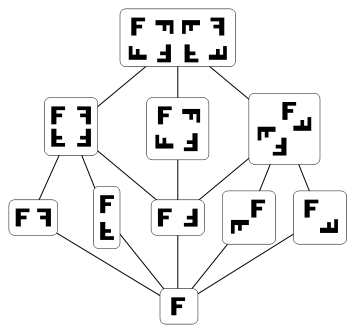
\includegraphics[height=2.1in]{D4_subgroups}
    \column{5cm} The lattice of subgroups of the dihedral group $D_4$,
    represented as groups of rotations and reflections of a plane figure. 
  \end{columns}
}

%% 9.
\frame[label=info]{
  \frametitle{...ok, but is it useful?}
  \uncover<2->{
  Lattice-theoretic information (about $\bSub[\bG]$) can be used to obtain
  group-theoretic information (about $\bG$).\\[4pt]
  \uncover<3->{
    {\bf Examples:} 
    \begin{itemize}
    \item  $\bG$ is locally cyclic if and only if $\bSub[\bG]$ is distributive.\\[4pt]
      % {\O}ystein Ore, ``Structures and group theory,'' {\it Duke Math. J.} (1937)
      Ore, ``Structures and group theory,'' {\it Duke Math. J.} (1937)
    }
    \uncover<4->{
    \item Similar lattice-theoretic characterizations exist for solvable and
      perfect groups.\\[4pt]
      % Michio Suzuki, ``On the lattice of subgroups of finite groups,'' {\it Trans. AMS.}
      % (1951) 
      Suzuki, ``On the lattice of subgroups of finite groups,''\\ {\it Trans. AMS} (1951) 
    \end{itemize}
  }
}
}

%% 10.
\frame[label=conglat]{
  \frametitle{$\bCon \bA$ is a lattice}
  \begin{itemize}
    % \item  Each $\theta \in \Con(\bA)$ is a subalgebra of the product algebra.
    %   \[ \therefore \quad \Con(\bA) \subseteq \Sub[\bA\times \bA]. \]
  \item<1->  The set $\Con(\bA)$, ordered by set inclusion, is a 0-1 lattice:
    \[
    \bCon \bA  = \langle \Con(\bA), \subseteq\rangle = \langle \Con(\bA), \meet, \join\rangle
    \]
%    \vspace{-5mm}
    \begin{itemize}
    \item<2-> The greatest congruence is the {\it all} relation
      \[\nabla = A\times A\]
    \item<3-> The least congruence is the {\it diagonal} 
      \[\Delta = \{(x,y)\in A\times A \, \vert \, x=y\} \]
    \item<4-> What are meet and join?
    \end{itemize}
  \end{itemize}
}

%\subsection{The FLRP}
\subsection{the finite lattice representation problem}
%% 11.
\frame[label=flrp]{
  \frametitle{The finite lattice representation problem}
  \begin{definition}[representable lattice]
    Call a finite lattice \alert{representable} if it is (isomorphic to)
    the congruence lattice of a finite algebra.
  \end{definition}
  \uncover<2->{%
    \begin{block}{The ($\leq$ \$1m) question}
      Is every finite lattice representable?\\[6pt]
    }
    \uncover<3->{%
      Equivalently, given a finite lattice \bL, does there exist\\
      a finite algebra \bA\ such that $\bCon \bA \cong \bL$?
    \end{block}
  }
  % }
}


%%%%%%%%%%%%%%%%%%%%%%%  SECTION: Groups %%%%%%%%%%%%%%%%%%%%%%%%%%%%%%%%%%%
\section{Groups}
\subsection{G-sets}
%% 12.
\frame[label=gsets]{
  \frametitle{What is a G-set?}
  Let $\bG=\langle G, \cdot, ^{-1}, 1_G\rangle$ be a group, $A$ a set.
  \uncover<2->{
    \begin{definition}[G-set]
      A \alert{G-set} is a unary algebra $\bA= \langle A, \overline{G} \rangle$,
      where $\overline{G} = \{\bar{g}: g\in G\}$, \\[4pt]$\overline{1_G} =
      \id_A$, and  $\overline{g_1} \circ \overline{g_2} = \overline{g_1 \cdot g_2}$, for all $g_i\in G$.
    \end{definition}
  }
  \uncover<3->{%
    \begin{definition}[stabilizer]
      For any $a\in A$, the \alert{stabilizer} of $a$ is the set
      \[
      \Stab(a) = \{g\in G \, \vert \, \bar{g}(a) = a\}
      \]
      \phantom{x}
    \end{definition}
  }
}

\frame[label=transgsets]{
  \frametitle{G-sets: basic facts and transitivity}
%  Let $\bA = \langle A, \overline{G}\rangle$ be a G-set.
  \uncover<2->{
    \begin{block}{Basic facts about the G-set $\langle A, \overline{G}\rangle$ (efts)}{
        \begin{itemize}
        \item<2->[1.] Each $\bar{g}\in \overline{G}$ is a permutation of $A$.
        \item<3->[2.] If $[a]$ is the subalgebra generated by $a\in A$, then
          \[  
          [a] = \{ \bar{g}(a) \, \vert \, g\in G\} = \text{ the \alert{orbit} of $a$ in $A$.}
          \]
        \item<4->[3.] The stabilizer $\bStab(a)$ is a subgroup of $\bG$.
        \end{itemize}
      }
    \end{block}
  }
  \uncover<5->{
    \begin{definition}[trasitive G-set]
      If $\bA = \langle A, \overline{G}\rangle$ has only one orbit, 
      we say $\bG$ \alert{acts transitively} on $\bA$, 
      % or $\bG$ is a \alert{transitive permutation group}, 
      or $\bA$ is a \alert{transitive G-set}.
    \end{definition}
    % define stabilizer
  }
}


%\subsection{The FTTG} 
\subsection{intervals in subgroup lattices}
%% 13.
\frame[label=fttg]{
  \frametitle{Fundamental theorem of transitive G-sets}
  % Main lemma on intervals in subgroup lattices}
  \begin{definition}[interval in a subgroup lattice]
    If \bG\ is a group and $\bH \in \Sub[\bG]$ is a subgroup, define
    \[
    [\bH, \bG] = \langle \{ \bK\in \Sub[\bG] \, \vert \, \bH \subseteq \bK\}, \subseteq \rangle
    \]
    Call $[\bH, \bG]$ an \emph{(upper) interval} in the lattice $\bSub[G]$.
  \end{definition}
  \uncover<2->{
    \begin{theorem}
      If $\bA = \langle A, \overline{G}\rangle$ is a transitive G-set, then
      for any $a\in A$,
      \[
      \bCon \bA \cong [\bStab(a), \bG]
      \]
    \end{theorem}
  }
}

%%%%%%%%%%%%%%  SECTION: Milestones %%%%%%%%%%%%%%%%%%%
\section{Milestones}
\subsection{the theorem of P\'alfy-Pudl\'ak}
%% 14.
\frame[label=pair]{
  \frametitle{A pair of groundbreaking results}
  \begin{theorem}[Pudl\'ak and T\r{u}ma, AU 10, 1980]
    A finite lattice can be embedded in $\Eq(X)$, for some finite $X$.
  \end{theorem}
\uncover<2->{
  \begin{theorem}[P\'alfy and Pudl\'ak, AU 11, 1980]
    The following statements are equivalent:
    \begin{itemize}
    \item[(i)] Any finite lattice is isomorphic to\\
      the congruence lattice of a finite algebra.
    \item[(ii)] Any finite lattice is isomorphic to\\
      an interval in the subgroup lattice of a finite group.
    \end{itemize}
  \end{theorem}
}
}

%% 15.
\frame[label=notPP]{
  \frametitle{The P\'alfy-Pudl\'ak theorem: what does it (not) say?}
%   \begin{theorem}[P\'alfy and Pudl\'ak, AU 11, 1980]
%     The following statements are equivalent:
%     \begin{itemize}
%     \item[(i)] Any finite lattice is isomorphic to\\
%       the congruence lattice of a finite algebra.
%     \item[(ii)] Any finite lattice is isomorphic to\\
%       an interval in the subgroup lattice of a finite group.
%     \end{itemize}
%   \end{theorem}
  \uncover<2->{
    \begin{block}{A quote from MathSciNet reviews}{} % \uncover<4->{(reviewer shall remain anonymous)}}{}
      {\it ``In AU 11, P\'alfy and Pudl\'ak proved that...a finite lattice is
      representable if and only if it occurs as an interval in the subgroup lattice
      of a finite group.'' }
      \\[4pt]
      \uncover<3->{
        \alert{False!} 
      }
    \end{block}
  }
  
}
\subsection{the seminal lemma of tct}
\frame[label=seminal]{
  \frametitle{The seminal lemma of tct}
  \begin{lemma}
      Let $\bA = \langle A, F\rangle$ be a unary algebra with 
      %$F$ a monoid, 
      $e^2=e\in F$.\\[4pt]
      Define $\bB = \langle B, G\rangle$ with
      \[
      B= e(A) \quad \text{ and } \quad G = \{ef\rvert_B : f\in F\}
      \]
      \uncover<2->{
      Then 
      \[
      \Con(\bA) \ni \theta \mapsto \theta \cap (B\times B) \in \Con(\bB)
      \]
      is a lattice epimorphism.
    }
  \end{lemma}
}

\frame[label=theorem1]{
  \frametitle{Consequence of the seminal lemma}
  \begin{theorem}
    Let $\bL$ be a finite lattice satisfying conditions (A), (B), (C).\\[4pt]
    Let $\bA = \langle A, F\rangle$ be a finite unary
    algebra of minimal cardinality such that $\bCon \bA \cong \bL$.\\[4pt]
    \uncover<2->{
      Then %(under certain conditions)
      %satisfies (A), (B), and (C), then 
      $\bA$ is a transitive G-set.
}
  \uncover<3->{
\[
\therefore \quad \bL \cong \bCon \bA \cong [\bStab(a), \bG]
\]
    }
  \end{theorem}
}


%%%%%%%%%%%%%%%%%%%%%%%%%%% SECTION: Summary %%%%%%%%%%%%%%%%%%%%%%%%%%%%%%%%%%%
\section*{Summary}
\frame[label=summary]{
  \frametitle<presentation>{Summary}

  % Keep the summary *very short*.
  \begin{itemize}
  \item<1->
    \underline{Problem}: Given a finite lattice $\bL$, does there exist a finite
    \phantom{\underline{Problem}:} algebra $\bA$ such that $\bL \cong \bCon \bA$?\\[4pt]
  \item<2-> It is generally believed the answer is no. 
  \item<3-> About 30 years ago P\'alfy and Pudl\'ak translated it into one
    for the group theorists, but still no answer...
  \end{itemize}
  
\uncover<4->{
  % The following outlook is optional.
%   \vskip0pt plus.5fill
   \begin{itemize}
   \item
    \underline{Outlook}: {\it bleak}
     \begin{itemize}
     \item<5->
       Something you haven't solved.
     \item<6->
       Something else you haven't solved.
     \end{itemize}
   \end{itemize}
}
}


\end{document}


%%%%%%%%%%%%%%%%%%%%%%%% END DOCUMENT %%%%%%%%%%%%%%%%%%%%%%%%%%%%%%%%%%%





\frame[label=]{
  \frametitle{Make Titles Informative.}
\end{frame}

\section{Groups}
\subsection{G-sets}
\frame[label=gsets]{
  \frametitle{Make Titles Informative.}
\end{frame}
\subsection{Main Lemma on intervals in subgroup lattices}
\frame[label=fttg]{
  \frametitle{Make Titles Informative.}
\end{frame}

\section*{Summary}

\frame[label=]{
  \frametitle<presentation>{Summary}

  % Keep the summary *very short*.
  \begin{itemize}
  \item
    The \alert{first main message} of your talk in one or two lines.
  \item
    The \alert{second main message} of your talk in one or two lines.
  \item
    Perhaps a \alert{third message}, but not more than that.
  \end{itemize}
  
  % The following outlook is optional.
  \vskip0pt plus.5fill
  \begin{itemize}
  \item
    Outlook
    \begin{itemize}
    \item
      Something you haven't solved.
    \item
      Something else you haven't solved.
    \end{itemize}
  \end{itemize}
\end{frame}



% All of the following is optional and typically not needed. 
\appendix
\section<presentation>*{\appendixname}
\subsection<presentation>*{For Further Reading}

\frame[label=]{[allowframebreaks]
  \frametitle<presentation>{For Further Reading}
    
  \begin{thebibliography}{10}
    
  \beamertemplatebookbibitems
  % Start with overview books.

  \bibitem{Author1990}
    A.~Author.
    \newblock {\em Handbook of Everything}.
    \newblock Some Press, 1990.
 
    
  \beamertemplatearticlebibitems
  % Followed by interesting articles. Keep the list short. 

  \bibitem{Someone2000}
    S.~Someone.
    \newblock On this and that.
    \newblock {\em Journal of This and That}, 2(1):50--100,
    2000.
  \end{thebibliography}
\end{frame}

\end{document}


\frame[label=]{
  \frametitle{Early Results}
  \uncover<1->{%
    \begin{block}{{\bf Theorem} (Gr\"{a}tzer and Schmidt 1963)}{}
      Every algebraic lattice is isomorphic to the congruence lattice of an algebra.
    \end{block}
  }
\note<1>{This shows that there is no lattice-theoretical condition stronger than
  algebraicity satisfied by all congruence lattices.}
\uncover<2->{%
  \begin{block}{What if the lattice is finite?}{}
  }
  \uncover<3->{%
    {\bf Problem:} Given a finite lattice \bL, does there exist a \emph{finite}
    algebra \bA\ such that $\bCon \bA \cong \bL$?
  }
  \uncover<4->{%
    \begin{itemize}
    \item status: \uncover<5->{open}
    \item age: \uncover<6->{40+ years}
    \item difficulty: \uncover<7->{\emph{what do you think?}}
    \end{itemize}
  \end{block}
}

\uncover<7->{%
  \begin{block}{{\it Representable} Lattices}{}
  }
  \uncover<8->{%
    Call a finite lattice {\bf representable} if it is the congruence lattice of a finite algebra.  
  \end{block}
}

\end{frame}



\frame[label=subgrouplattice]{
\frametitle{The Lattice $\bSub[\bG]$}
\begin{block}{}
  The {\it subgroup lattice} of a group \bG\ is denoted
\[
\bSub[\bG] = \langle \Sub[\bG], \subseteq \rangle = \langle \Sub[\bG],\meet, \join\rangle 
\]
The elements are the subgroups of \bG, partially ordered by set inclusion.
\end{block}

\begin{block}{}
For subgroups $H, K \leq G$, 
\begin{itemize}
\item The meet is intersection: 
\[
H\meet K = H\cap K
\]
\item The join is the subgroup generated by the union:
\[
H\join K = \bigcap \{J\leq G \, \vert \, H\cup K \subseteq J\}
\]
\end{itemize}  
\end{block}
}


% Structuring a talk is a difficult task and the following structure
% may not be suitable. Here are some rules that apply for this
% solution: 

% - Exactly two or three sections (other than the summary).
% - At *most* three subsections per section.
% - Talk about 30s to 2min per frame. So there should be between about
%   15 and 30 frames, all told.

% - A conference audience is likely to know very little of what you
%   are going to talk about. So *simplify*!
% - In a 20min talk, getting the main ideas across is hard
%   enough. Leave out details, even if it means being less precise than
%   you think necessary.
% - If you omit details that are vital to the proof/implementation,
%   just say so once. Everybody will be happy with that.

%     {\it Example:} $\bSub(V)$, the subspaces of a vector space.

% \frame[label=]{
%   \frametitle{Some History...}
%   \begin{itemize}
%   \item[pjm 82] {\bf Theorem (Freese, Lampe, Taylor 1979)} If $V$ is an infinite vector space
%     over an uncountable field $F$, then $\bCon(\bA)\cong \bSub(V)$ implies $\bA$ has at least $|F|$ operations.\\[4pt]
% %    {\it Key point:} As $V$ is infinite, the largest element or ``unit'' of $\bSub(V)$ is not
% %    compact. The next result shows that a compact unit is essential.
%   \item[pjm 103] {\bf Theorem (Lampe 1982)} Every algebraic lattice with compact unit is
%     isomorphic to the congruence lattice of some groupoid. 
%   \end{itemize}
% \end{frame}
% % Ji\v{r}\'i 
% %P\'eter 



\frame[label=conglat2]{
  \frametitle{The Lattice of Congruence Relations}
  \begin{itemize}
  \item $\bCon \bA$ is a complete lattice.
  \item The \emph{compact} elements of $\bCon \bA$ are the finitely generated congruences.
  \item $\bCon \bA$ is an \emph{algebraic} lattice.
  \end{itemize}
Conversely, Gr\"{a}tzer and Schmidt (1962) proved that any algebraic lattice is a
congruence lattice.
  \begin{itemize}
  \item 
  \end{itemize}
  Again there is a converse: By a theorem of , every algebraic lattice is isomorphic to Con(A) for some algebra A.
